\documentclass[10pt, a4paper,english,spanish,hidelinks]{article}
\usepackage{amsmath}
\usepackage{amsfonts}
\usepackage{amssymb}
\usepackage{caratula}
\usepackage[spanish, activeacute]{babel}
\usepackage[usenames,dvipsnames]{color}
\usepackage[width=15.5cm, left=3cm, top=2.5cm, height= 24.5cm]{geometry}
\usepackage{graphicx}
\usepackage[utf8]{inputenc}
\usepackage{listings}
\usepackage{multicol}
\usepackage{subfig}
\usepackage{float}
\usepackage{color,hyperref}


\usepackage{listings}
\usepackage{babel}
\usepackage{url}
\usepackage{lscape}
\parindent = 15 pt
\parskip = 11 pt

\usepackage{fancyhdr}
\usepackage{hyperref}
\usepackage{amsmath}
\usepackage{amsfonts}
\usepackage{amssymb}
\usepackage[utf8]{inputenc}
\usepackage{graphicx}
\usepackage{caption}
\usepackage{color}
\usepackage{appendix}
\usepackage{fancyhdr}


\materia{Base de Datos}

\titulo{Trabajo Práctico 2}
\fecha{13 de Junio de 2014}
\grupo{Bobby Tables}
\integrante{Mancuso Emiliano}{597/07}{emiliano.mancuso@gmail.com}
\integrante{Mataloni Alejandro}{706/07}{amataloni@gmail.com}
\integrante{Gauder María Lara}{027/10}{marialaraa@gmail.com}
\integrante{Reartes Marisol}{422/10}{marisol.r5@hotmail.com}


\include{templates}

\begin{document}
\pagestyle{myheadings}
\maketitle
\markboth{Base de Datos}{Análisis de distribución de datos}

\thispagestyle{empty}
\tableofcontents

\setcounter{section}{-1}

\newpage
\section{Ejemplos de la vida cotidiana}
Para comenzar, se presentan ejemplos de la vida cotidiana, es decir, ejemplos reales, para la distribución normal y uniforme de datos. 

\subsection{Distribución normal}
\begin{itemize}
\item Ejemplo 1: Un ejemplo de la vida real cuya información presenta una distribución normal, puede ser el de los datos metereológicos correspondientes a temperaturas, lluvias, etc. 

\item Ejemplo 2: Otro ejemplo es el de la vida media de un producto electrónico. Al fabricarlo, se espera un tiempo de vida útil, pero el mismo puede ocurrir ser menor o mayor según el uso que se le de, mientras que el esperado en general se cumplirá. 

\item Dataset: Luego de analizar diferentes casos, se encontró que la temperatura desde el año 1911 al 1972 en el mes de Enero, presentan una distribución normal de los datos. A continuación se presenta la tabla con los datos \footnote{http://infometeoba.blogspot.com.ar/}:

\begin{table}[htdp]
  \begin{center}
    \begin{tabular}{|c|c|c|c|c|c|c|c|c|c|c|c|c|c|c|c|} \hline
       Año  & 1911 & 1913 & 1915 & 1916 & 1921 & .. & 1966& 1968& 1969& 1970& 1971& 1972 \\ \hline
       Temperatura Mínima & 16,8 & 15,9 & 17 & 17 & 15,8 & .. & 19 & 18,6 & 18,9 & 19,4 & 18,5 & 20,2 \\ \hline
    \end{tabular}
  \end{center}
\end{table} 

Además, se observa a continuación el gráfico por el cual se determina si efectivamente el dataset cumple con una distribución normal.

\begin{figure}[h!]
  \centering
  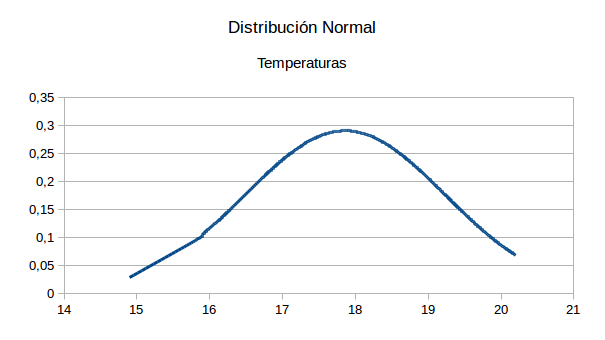
\includegraphics[width=0.7\textwidth]{./imagenes/DatasetNormal.png}
  \caption{}
\end{figure}

Como se puede observar, el dataset cumple con una distribución normal de los datos. 


\end{itemize}

\subsection{Distribución Uniforme}
\begin{itemize}
\item Ejemplo 1: En la vida real se puede observar que las edades de las personas de cierta ciudad presentan una distrubución informe. 

\item Ejemplo 2: Otro caso a tener en cuenta, que respeta una distribución uniforme es el de las frecuencias en las que un tren en Buenos Aires arriba a una estación. Se debe tener en cuenta únicamente el horario en el que el tren funciona. 

\item Dataset: Se encontraron la cantidad de nacimientos agrupados por fecha en google big query\footnote{https://bigquery.cloud.google.com/}:

Graficamos estos datos para corrobar la distribución de los mismos

\begin{figure}[h!]
  \centering
  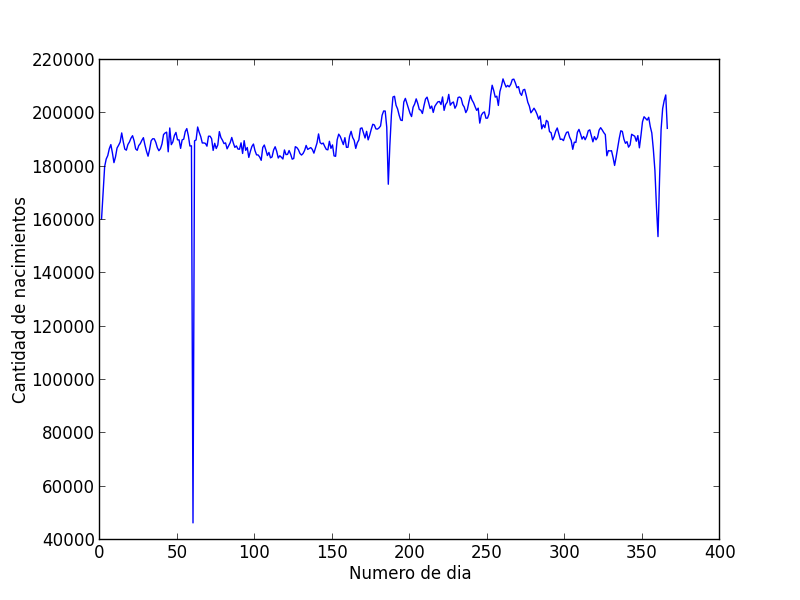
\includegraphics[width=0.7\textwidth]{./imagenes/ejemplo_dia_nacimiento.png}
  \caption{}
\end{figure}

  Como se puede observar los datos siguen una distribución uniforme. Lo que nos 
llamo la atencion fue el pico en el dia 60, pero nos dimos cuenta que 
corresponde al 29/02 ya que era un año bisiesto. 

\end{itemize}

\newpage
\section{Análisis de métodos}
Tanto Classic Histogram como Distrbution Steps son estimadores de aquellas tuplas que satisfacen una condición dada. Se puede realizar una búsqueda por aquellas tuplas que cumplan una condición de igualdad, por menor o menor igual y por mayor o mayor igual a cierto valor. Los estimadores son utilizados en las bases de datos en el proceso de seleccionar un plan de ejecucion óptimo 
al momento de realizar una consulta.

Además, se desarrolla un estimador propio al que se lo denomina \textbf{Group Histogram}. El mismo cumple con la misma función que los otros dos estimadores, pero presenta un rendimiento diferente. 

Son varios los factores que se involucran en el cálculo de estimadores. Alguno de ellos
son la precisión, la cantidad de información que contenga la base de datos, los errores
en la estimación, el espacio que consume el estimador y la estructura para consultar la
información requerida. Cada uno de estos factores se ajustan al modificar algunas variables
que son pasadas por parámetros a los algoritmos de los estimadores.

Las variables en cuestión Las variables en cuestión para el \textbf{Classic Histogram] y el \textbf{Distribution Steps} son:
\begin{itemize}
\item La tabla a la que se desea realizar las consultas,
\item Una columna,
\item Una variable denominada PARAM que representan la cantidad en la que se va a agrupar
los datos de la base, es decir, la cantidad de steps.
\end{itemize}


Por otro lado, el \textbf{Group Histogram} requiere las siguientes variables:
\begin{itemize}
	\item La tabla a la que se desea realizar las consultas,
	\item Una columna,
  	\item Size, que representa la cantidad de steps,
  	\item Threshold, es decir un máximo error permitido.
\end{itemize}

Los \textit{steps} denotan la cantidad en la que se dividen los conjuntos de datos.
Por lo tanto, es claro que al aumentar el valor de steps se aumenta la presición y se disminuye el error en la estimación.

El beneficio que aporta el estimador \textbf{Distrbution Steps} podrá ser observado al compararlo
con \textbf{Classic Histogram} y evaluando diferentes factores. Principalmente se tiene en cuenta
el costo temporal y espacial de la construcción de las estructuras requeridas por el
estimador, el costo temporal de la consulta y el error que comete en la misma.

Luego, se realizaran experimentos con el objetivo de comparar los tres estimadores nombrados y observar sus comportamientos. 
\newpage
\subsection{Performance}
Para entender el funcionamiento del \textbf{Classic Histogram} y del \textbf{Distribution Steps}, se creó el siguiente caso simple de prueba:

\begin{table}[htdp]
  \begin{center}
    \begin{tabular}{|c|c|c|c|c|c|c|c|c|c|c|c|c|c|} \hline
       Número  & 0 & 1 & 2 & 3 & 4 & 5 & 6 & 7 & 8 & 9 & 10 & 11 & 12 \\ \hline
       Cantidad & 1 & 1 & 0 & 1 & 12 & 1 & 0 & 2 & 0 & 1 & 0 & 0 & 1 \\ \hline
    \end{tabular}
  \end{center}
\end{table}


Se espera que \textbf{Distrution steps} presente un mejor rendimiento pues, como indica el \textit{paper} (Piatetsky),
se soluciona el problema existente en \textbf{Classic Histogram}, manejando la altura
de los bins.

\begin{figure}[h!]
  \centering
  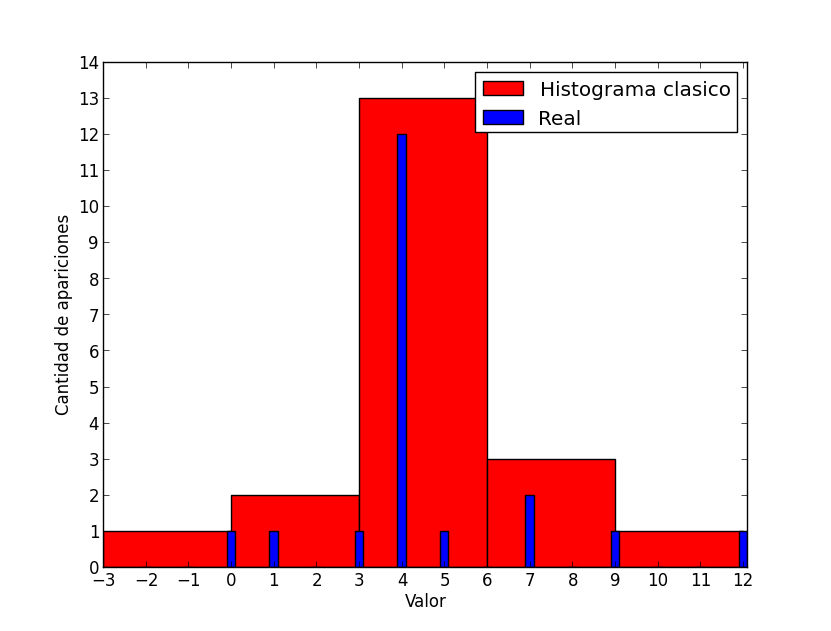
\includegraphics[width=0.7\textwidth]{./imagenes/ejb1_ejemplo_classic_y_real.png}
  \caption{Comparación: Classic Histogram vs. Resultado Exacto}
\end{figure}


Tomando como ejemplo la $selectividad de 5$.
En la \textit{Figura 1} se observa que la selectividad es de $0.65$, debido a que queda agrupado junto
con $4$, que que aparece muchas veces en el resultado. Sin embargo, los datos reales indican que deberia ser $0.05$, ya que tiene menor cantidad de apariciones.

Como se puede ver, este es un caso \textbf{no favorable} para \textbf{Classic Histogram}. Por otro lado, se puede denotar la ventaja de controlar la altura de los bins.

\newpage
\begin{figure}[h!]
  \centering
  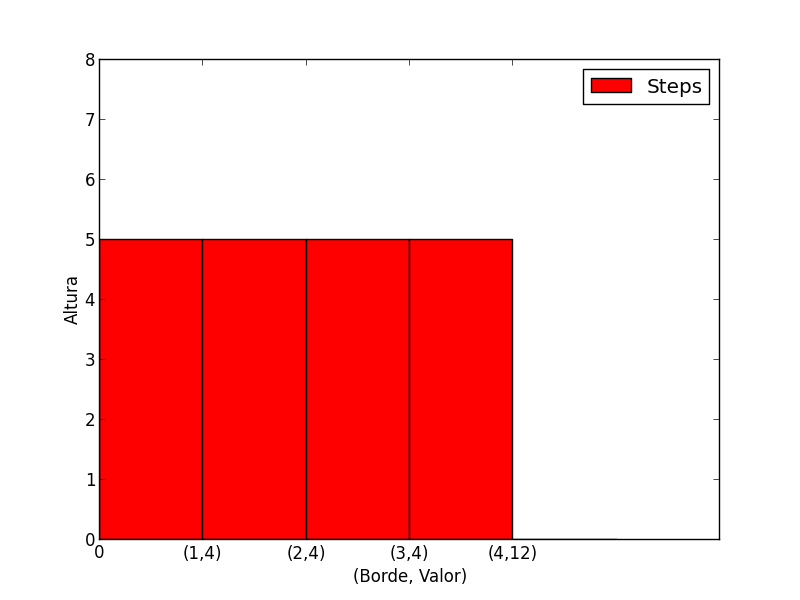
\includegraphics[width=0.6\textwidth]{./imagenes/ejb1_ejemplo_steps.png}
  \caption{Distribution Steps}
\end{figure}


Para el mismo ejemplo utilizado anteriormente, se examina la $selectividad de 5$ nuevamente con el estimador Distribution Steps.
Se podrá observar, que la selectividad es de $0.25$. Si bien también se desvia del
valor real ($0.05$), la diferencia del error es significativa comparada con el estimador Classic Histogram.


Basándose en el ejemplo planteado, se observa que el comportamiento de los distintos estimadores
depende de la distribición de los datos.
Por ejemplo, cuando los datos están agrupados, \textbf{Distribucion Steps} brinda un menor
error en la estimación pero, cuando los datos estan dispersos el error del estimador es
mucho mayor que el que presenta \textbf{Classic Histogram}.


\subsection{Generación casos de prueba}
Los casos de prueba que se van a utilizar para el análisis del comportamiento de los
estimadores, se generarán de manera aleatoria. Se define una función que genera números
aleatorios que siguen una distribucion normal o uniforme.

\subsection{Factores}

Debido a la estructura que se utiliza para construir los estimadores y el algoritmo de
construcción de los mismos, se podrá afirmar que:

\subsubsection{Classic Histogram}
% Usamos un diccionario
\begin{itemize}

\item Costo de creación de estimador:
\begin{equation}
O(b * n + n )
\end{equation}
\begin{equation}
O(b * n)
\end{equation}

Siendo \textit{n} la cantidad total de tuplas existentes en la base de datos.
Por el otro lado, \textit{b} representa el valor pasado en \textbf{PARAM}.
Como se recorre toda la tabla por cada dato que se requiere para la tabla del estimador,
se deberá considerar un costo de $b * n$. Por otro lado, también se requiere almacenar en
la estructura del estimador, el máximo, mínimo y la cantidad total de tuplas, lo cual es
una búsqueda que realiza el motor de bases de datos en tiempo lineal.

\item Costo espacial del estimador:
\begin{equation}
O(2 * b + 3 ) \\
\end{equation}
\begin{equation}
O(2 * b)
\end{equation}
Se utiliza un diccionario que presenta un costo espacial del valor pasado en PARAM por dos,
ya que por cada bin se almacen dos valores más (la cantidad y el acumulado hasta ese valor).
Por otro lado, se requere almacenar el máximo, mínimo y la cantidad total.

\item Costo de consulta:
\begin{equation}
O(1)
\end{equation}
Lo único se se requere es el acceso al diccionario, lo cual presenta un costo constante.

\end{itemize}
\subsubsection{Distribution Steps}
% Usamos un Array

\begin{itemize}

\item Costo de creación del estimador:

\begin{equation}
O(n*log(n) + n + n) => O(n*log(n))
\end{equation}

El algoritmo consiste en el ordenamiento de las tuplas de acuerdo a la columna pasada por
parámetro. El ordanamiento lo realiza el motor de la base de datos en costo $O(n*log(n))$.
Por otro lado se deberá calcular el máximo, mínimo y total de tuplas existentes en la base.

\item Costo espacial del estimador:

\begin{equation}
O(b + 1) => O(b)
\end{equation}

Se requiere unicamente almacenar un array con las tuplas que se encuentran en las distintas
posiciones de los steps. Además, se deberá almacenar la cantidad de tuplas totales
existentes en la tabla pasada por parámetro.

\item Costo de consulta:

\begin{equation}
O(n)
\end{equation}

Tanto para una búsqueda por igualdad o por menor, se deberá recorrer el array buscando
el valor de tupla deseado.

\end{itemize}



\subsubsection{Distribution Group}

\begin{itemize}

\item Costo de creación de estimador:
Como es una modificación del \textbf{Classic Histogram}, el costo de creación no cambia.

\begin{equation}
O(b * n)
\end{equation}

\item Costo espacial del estimador:

En caso promedio, se comporta como \textbf{Classic Histogram}
\begin{equation}
O(b)
\end{equation}

Pero en el caso que el \textbf{threshold} sea muy bajo, o la varianza de la distribucion de los datos sea muy alta, crea un bin por cada valor. Esto dejaria un costo de

\begin{equation}
O(2 * n) => O(n)
\end{equation}


Se utiliza un diccionario que presenta un costo espacial del valor pasado en PARAM por dos,
ya que por cada bin se almacen dos valores más (la cantidad y el acumulado hasta ese valor).
Por otro lado, se requiere almacenar el máximo, mínimo y la cantidad total.


\item Costo de consulta:
\begin{equation}
O(1)
\end{equation}
Lo único se se requere es el acceso al diccionario, lo cual presenta un costo constante.
\end{itemize}


\subsection{Impacto en la variación de parámetros.}
A continuación, analizaremos el impacto de la variación de los parámetro para los estimadores y su consecuencia. En primer lugar, observaremos el comportamiento de \textbf{Classic Histogram|.

Como se explicó anteriormente, el \textbf{param} indica la cantidad de bins que generamos. Se supone que, cuando \textbf{param} toma un valor mas grande, disminuye el error en la estimación,
pues agrupa menor cantidad de valores por \textit{bin}.

Además, la distribución de los datos no influencia en el resultado. El histograma puede tener un menor error con una determinada distribución, pero la cantidad de
\textit{bins} se supone que produciría una reducción del error más significativa.

Se observa el siguiente gráfico que presenta el error promedio que comete el estimador, variando
la cantidad de \textit{bins}.

\begin{figure}
  \centering
  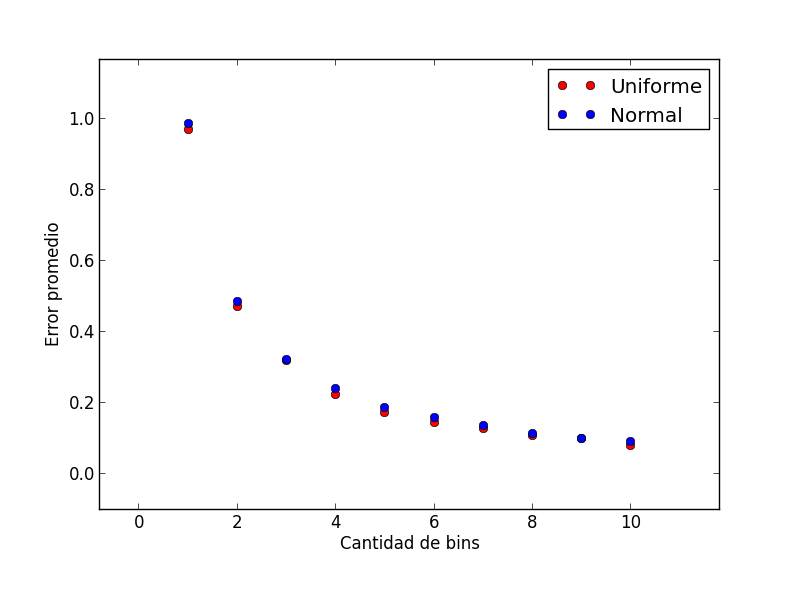
\includegraphics[width=0.7\textwidth]{./imagenes/ejb2_classic_parameter_variation.png}
  \caption{Classic Histogram - Variación del parámetro}
\end{figure}

\newpage

Como se esperaba, se observa una mejora a medida que se agranda la variable \textbf{param}.
Esto ocurre porque al aumentar la variable, se separan mejor los casos y, entonces se genera una estimación más precisa.
Sin embargo, por cada incremento de \textit{bin}, el costo espacial se incrementa pues se requiere
más espacio de memoria para almacenar las estadisticas.

Si implementamos que $param \rightarrow n$ (siendo $n$ la cantidad de valores distintos), nos
resultaría una estimación perfecta, pero con un costo muy alto, tanto espacial como computacional.

En segundo lugar, analizamos las consecuencias de variar la cantidad de steps en Distribution Steps. Para este estimador, partimos con una suposicion similar, pues la diferencia es que mientras
más \textit{steps} se crean, más chicos son los \textit{bins} que agrupan valores.


Se puede ver el siguiente gráfico, que muestra el error promedio que comete el histograma variando
la cantidad de \textit{bins}.

\newpage
\begin{figure}
  \centering
  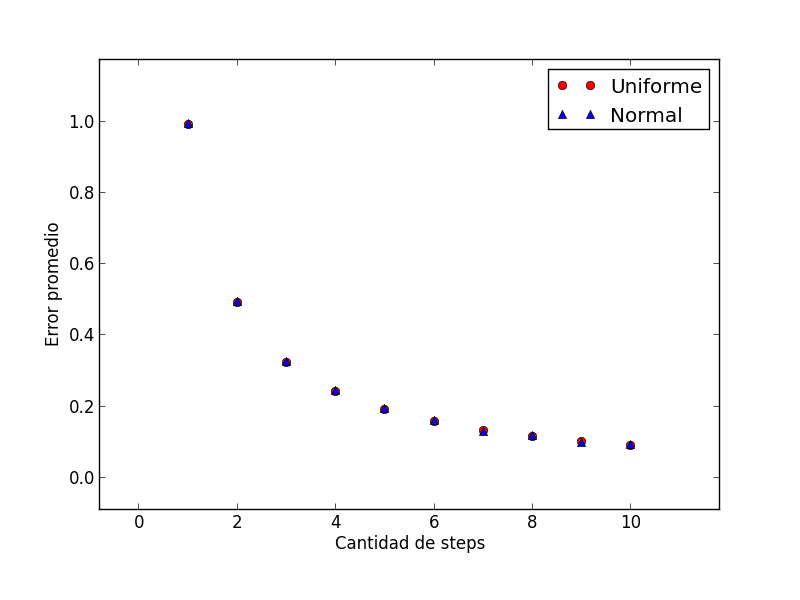
\includegraphics[width=0.7\textwidth]{./imagenes/ejb2_step_parameter_variation.png}
  \caption{Distribution Steps - Variación del parametro}
\end{figure}

Nuevamente, nuestra hipótesis es confirmada. El costo espacial y computacional también se incrementa al aumentar la 
la cantidad de \textit{steps}.

Por último, observamos el comportamiento para el estimador \textbf{Group Histogram}. 
Como este estimador consiste en una modificación de \textbf{Classic Histogram}, se debería obtener la misma
conclusión al variar el \textbf{size}, que es el equivalente de \textbf{params} en el estimador \textbf{Classic}.

Por lo tanto, se deberá ver como evoluciona la estimacion cuando se modifica el
\textbf{threshold}, es decir aumentando y disminuyendo el maximo error permitido.
Se espera que, a medida que se achica el \textbf{threshold}, la selectividad es mas precisa.

El siguiente gráfico muestra el \textit{máximo error} que comete el estimador
al variar el \textbf{threshold}.
\newpage
\begin{figure}
  \centering
  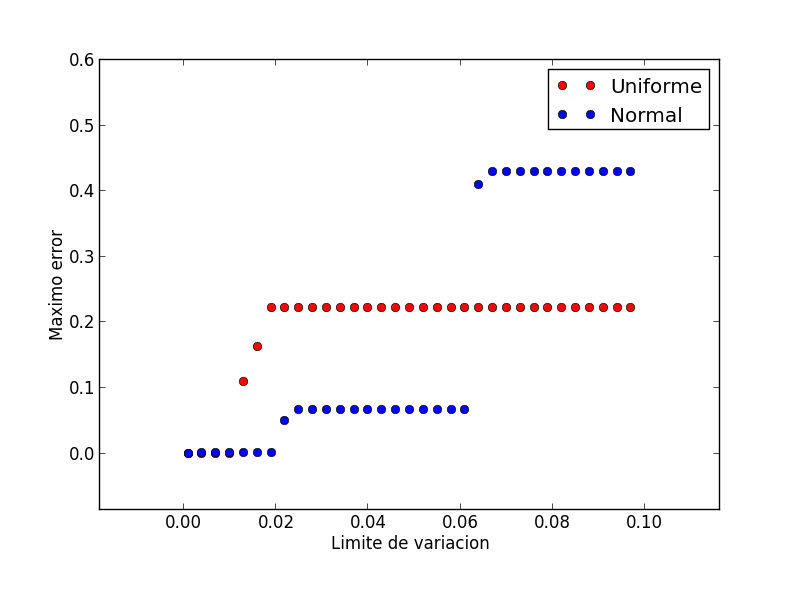
\includegraphics[width=0.7\textwidth]{./imagenes/ejb2_group_parameter_variation.png}
  \caption{Distribution Group - Variacion del threshold}
\end{figure}


En el caso de la distribución uniforme el máximo error llega a un
techo y no sigue creciendo. No se supuso desde el principio, pero cobra sentido si
se recuerda que los datos provienen de una distribución uniforme, donde la varianza no es
grande. Por eso sólo podemos apreciar las grandes mejoras con un \textbf{threshold} muy pequeño.

Para la distribución normal, el gráfico muestra como mejora la precisión o como se pierde
para los distintos valores del \textbf{threshold}. Se debería recordar, que una vez cruzado el
\textbf{threshold} se define un \textit{bin} por cada valor distinto, lo cual genera una mayor
precision pero aumenta la memoria consumida por la estructura y, al mismo tiempo, el tiempo
consumido para generarla.


\subsection{Impacto de acuerdo a la distribución de los datos.}
\subsubsection{Distribución Uniforme}

Se parte con una base de datos cuya información cumple con una distribución uniforme.

\begin{figure}[h!]
  \centering
  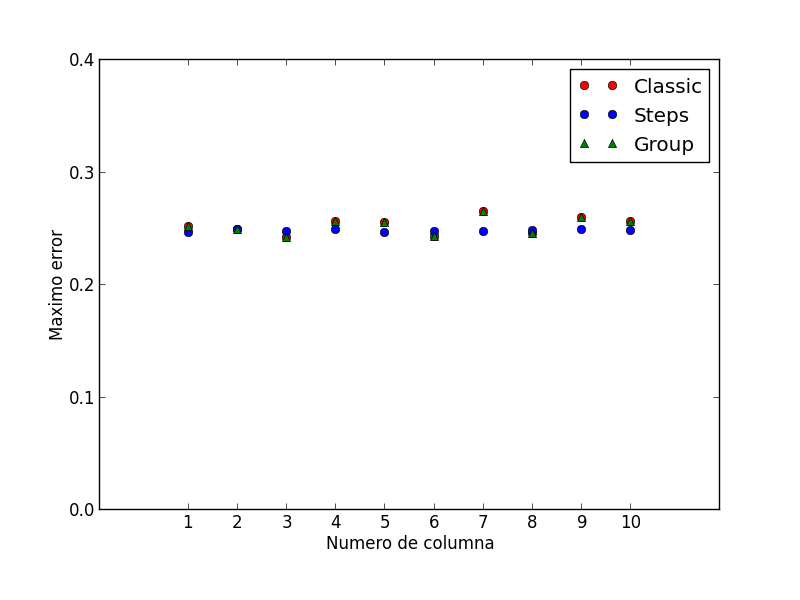
\includegraphics[width=0.7\textwidth]{./imagenes/ejb3_uniforme.png}
  \caption{Comparacion Classic, Step y Gruop para datos con distribución uniforme}
\end{figure}

\newpage
Con respecto al error de factor en la estimación, ambas estimaciones no difieren
significativamente en sus resultados. Dado que al tener los datos distribuidos de forma
uniforme, la probabilidad de cada tupla es $1/n$, siendo $n$ la cantidad total de tuplas de la tabla.

Debido a que se los compara con igual cantidad de steps, entonces la altura, en el caso de
\textbf{Classic Histogram}, y el ancho, en el \textbf{Distribution Steps}, son similares.
En el caso de \textbf{Group Histogram}, al ser una especializacion del Classic, tambien tiene
una altura similar.

Sin embargo, teniendo en cuenta el factor de costos de creación, el estimador
\textbf{Distribution Steps} es más costoso. El motivo principal es debido al ordenamiento
de los datos antes de construir el histograma requerido. Luego sigue el \textbf{Group Histogram}
pues requiere \textit{bins} particulares para los algunos elementos. Y por último se encuentra el \textbf{Classic Histogram}.

En conclusión, para datos que cumplen una distribución uniforme, sugerimos implementar
\textbf{Classic Histogram}, debido al menor costo de construcción del histograma.


\subsubsection{Distribución Normal}

A partir de una base de datos que la información que sigue una distribución normal se observan los siguientes resultados. Se realizaron experimentos modificando la varianza para observar el comportamiento de los tres estimadores.

Se realizaron diversos graficos comparandolos en simultáneo teniendo en cuenta el parametro dicho. 
A continuacion se presenta un ejemplo con una varianza igual a $0,05$. 

\begin{figure}[h!]
  \centering
  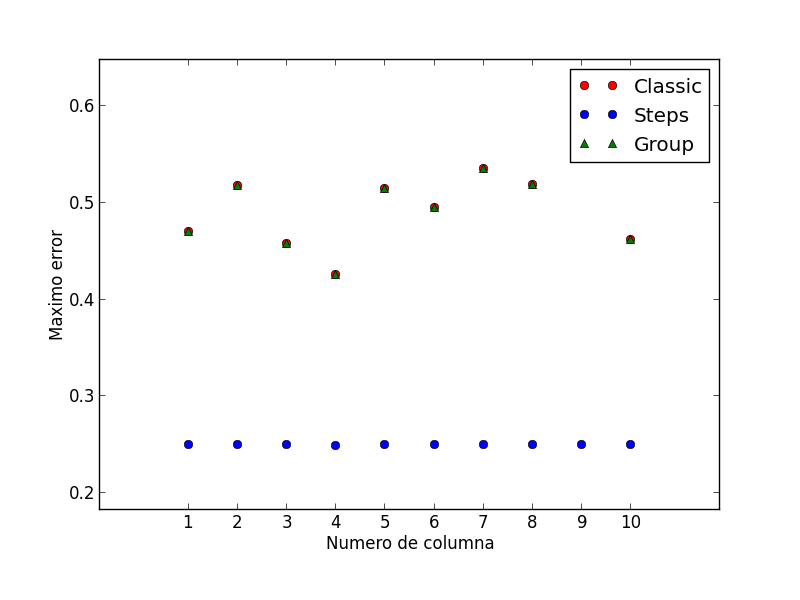
\includegraphics[width=0.7\textwidth]{./imagenes/ejb2_normal_t_005.png}
  \caption{Comparacion Classic vs. Step para distribucion normal}
\end{figure}

Como se puede ver, con una varianza chica, el error maximo es muy bajo en el estimador de \textbf{Distribution Steps}. En cambio, para \textbf{Classic Histogram} y \textbf{Group Histrograms} es más alto, aunque similar entre si. Esto se debe a que los resultados de \textbf{Gruop Histogram} son muy similares con respecto a \textbf{Classic Histogram} si no se acepta un error alto, ya que no se agregan bins. De esta manera no se puede notar la mejora del estimador.


Luego se presenta un experimento realizado con una varianza igual a $0,03$. 
\newpage
\begin{figure}
  \centering
  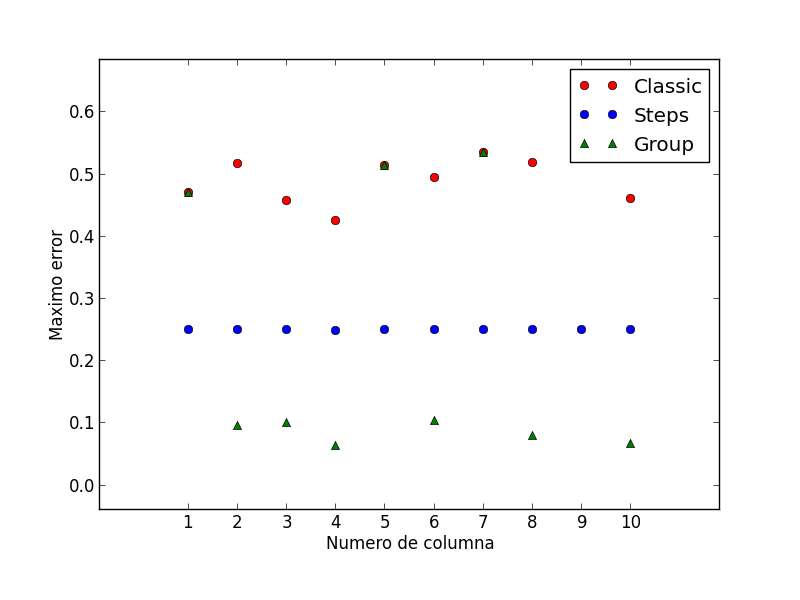
\includegraphics[width=0.7\textwidth]{./imagenes/ejb2_normal_t_003.png}
  \caption{Comparacion Classic vs. Step para distribucion normal}
\end{figure}

Con respecto al grafico anterior se puede observar una diferencia del máximo error para algunas columnas en el estimador \textbf{Group Histogram}. En los otros dos estimadores el error máximo sigue siendo similar ya que el cambio en la varianza no modifica sus resultados. 

La diferencia en \textbf{Group Histograms} se debe a que al disminuir la varianza se le esta indicando al algoritmo que el error maximo debe ser menor. Por lo tanto el estimador generara un mayor numero de bins aumentando asi la precision en los calculos. No ocurre una mejora para todas las columnas, ya que la varianza no es lo suficientemente baja. 

Por lo tanto, para el estimador \textbf{Group} es importante conocer la varianza de la distribución, pues nos
basamos en ella para encontrar un error aceptable. Es decir, el estimador ofrece una mejora al \textbf{Classic Histogram} cuando la distribución de los datos tiene un valor elevado de varianza.

A continucacion, se muestra otro grafico con una varianza de $0.01$
\newpage
\begin{figure}
  \centering
  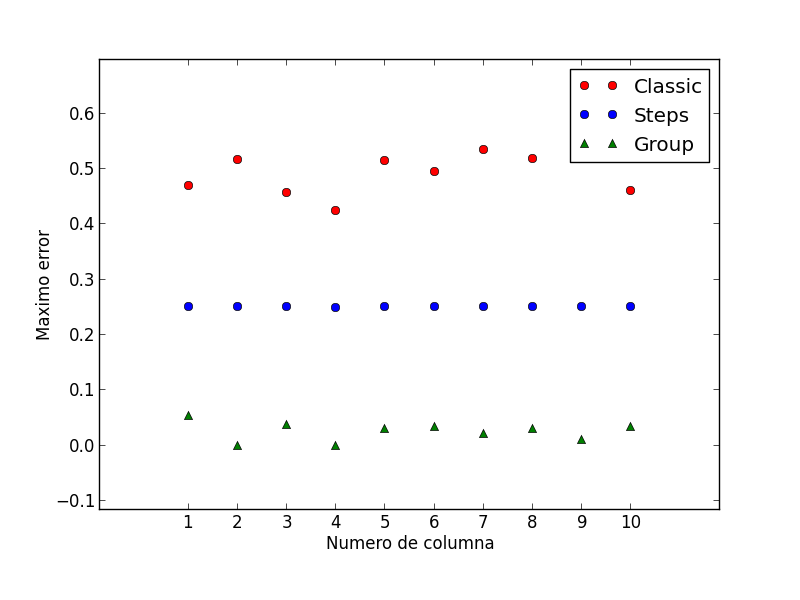
\includegraphics[scale=0.6]{./imagenes/ejb2_normal_t_001.png}
  \caption{Comparacion Classic vs. Step para distribucion normal}
\end{figure}

La diferencia con el grafico anterior es notoria con respecto a Group Histogram. Esto se debe a que la varianza pasa por parametro es lo suficientemente baja para que se genere una mejora en todas las columnas de la base de datos. 



\newpage

\section{Datasets}

\begin{figure}
  \centering
  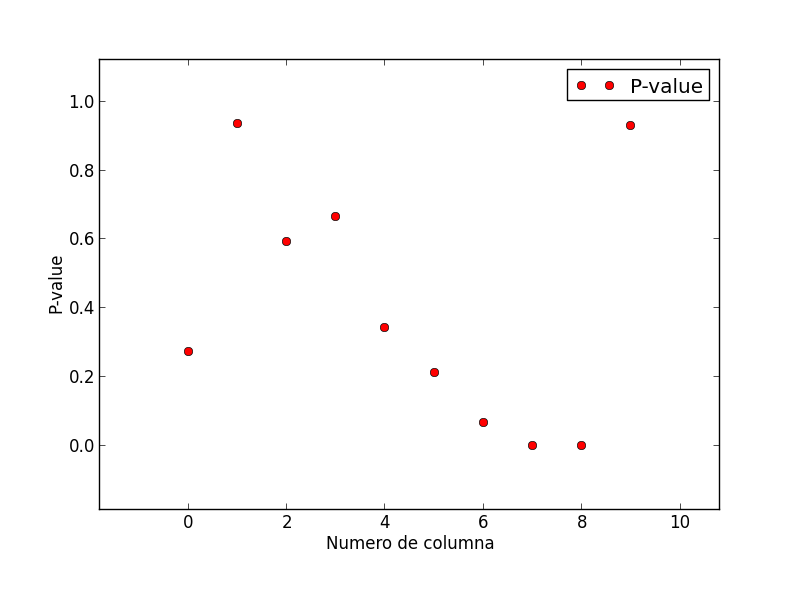
\includegraphics[scale=0.6]{./imagenes/ejc1_p_100.png}
  \caption{Student Test apareado}
\end{figure}


El \textit{valor p} nos muestra la probabilidad de haber obtenido el resultado si suponemos que la hipótesis nula es cierta. Si el \textit{valor p} es inferior a $0.1$ nos indica que lo más probable es que la hipótesis de partida sea falsa, es decir, que las dos muestras difieren por mucho.

\newpage

\subsection{Distribution Steps - Cota de error}

Para verificar las cotas propuestas por los Autores, tomamos tres diferentes casos:


\begin{table}[htdp]
  \begin{center}
    \begin{tabular}{|c|c|} \hline
       Steps & Cota \\ \hline
       2  & 0.5 \\ \hline
       5  & 0.2 \\ \hline
       10 & 0.1 \\ \hline
    \end{tabular}
  \end{center}
\end{table} 


Utilizando el histograma con estos parametros, las cotas, respectivamente, son:

\begin{figure}
  \centering
  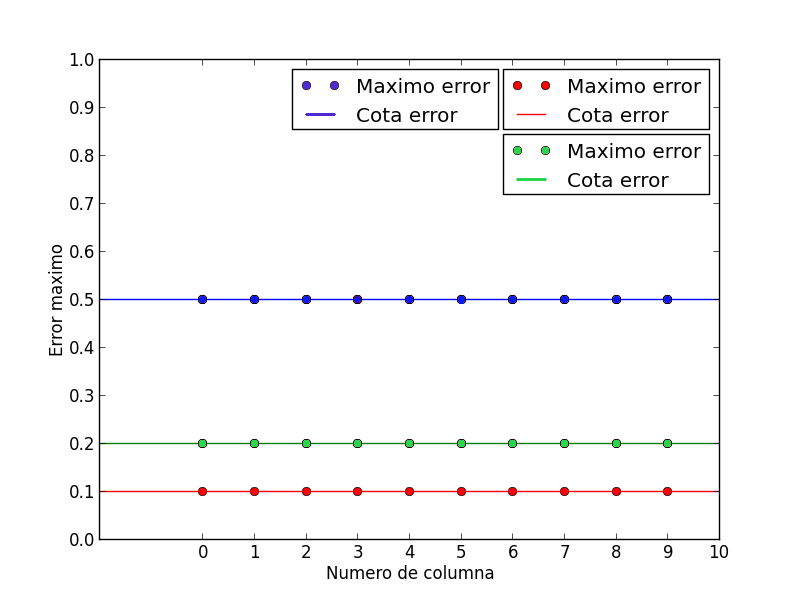
\includegraphics[scale=0.6]{./imagenes/ejc2_cota_juntos.png}
  \caption{Cotas de error - Distribution Steps}
\end{figure}

En la \textit{figura 12} detallamos los \textit{errores maximos} por cada columna de la Base de Datos de prueba, y a su vez, trazamos la cota de error esperada.
Como bien dicen los Autores, se cumple la cota $1/s$.


\subsection{Variacion}

Luego de haber hecho un analisis sobre las estructuras, la complejidad, consumo de memoria, etc, nos falta comparar la performance de este Histograma.

Dada la base de datos de la catedra, construimos por cada columna el histograma variando los \textit{steps}. Al mismo tiempo, calculamos el error promedio cometido por la estimacion y lo volcamos en el siguiente grafico.

\begin{figure}
  \centering
  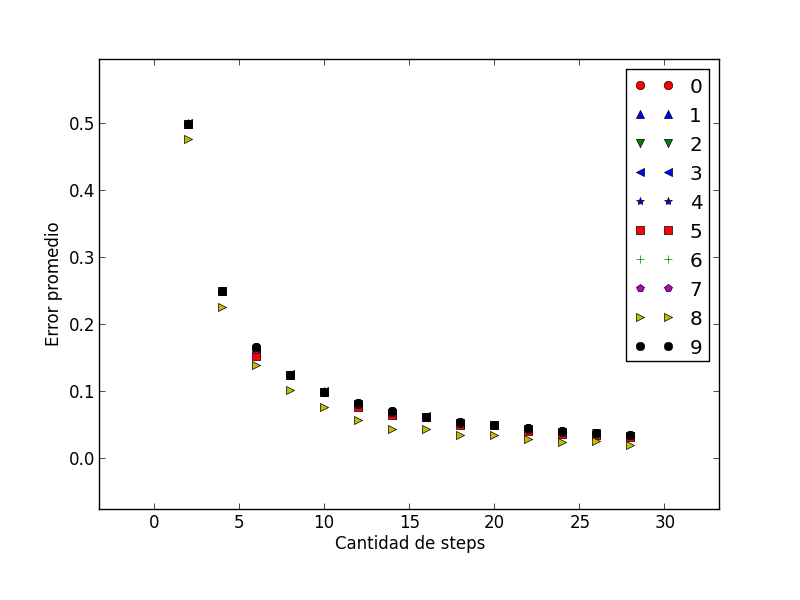
\includegraphics[scale=0.6]{./imagenes/ejc2_variacion.png}
  \caption{Variacion}
\end{figure}


Con los datos de la catedra, podemos concluir lo mismo que anteriormente. A medida que incrementamos la cantidad de steps del histograma, el error promedio o \textit{performance} mejora. De hecho, se ve claramente como la curva es logaritmica y se corresponde con la cota $1/s$

\end{document}